%----------------------------------------------------------------------------------------
%	CHAPTER 3: Ripa Exchange
%----------------------------------------------------------------------------------------

\chapterimage{chapter_head_3_Singapore.jpg} % Chapter heading image

\chapter{L'Exchange Ripa}
Ripa Exchange è un crypto asset marketplace implementato seguendo i più avanzati standard industriali seguendo il principio
``\textit{open source, sicuro ed efficiente}''. Ripa Exchange si prefigge di servire come piattaforma sicura, UI responsive, 
personalizzabile, facile da usare per gli imprenditori in questo settore abbracciando i principi Open Source e la fiducia pubblica.\\\\
Ripa Exchange è implementato utilizzando il framework Ruby on Rails ed altre tecnologie all'avanguardia e sarà migrato verso
un exchange ibrido-decentralizzato dove tutti gli exchange nella rete Ripa condivideranno la stessa liquidità grazie alla tecnologia R.L.S.P..

\section{Mission}
\begin{quotation}
	``\textit{La nostra mission è di costruire il crypto asset marketplace migliore al mondo con un trading engine ad alte prestazioni 
	e sicuro abbastanza da poter essere utilizzato dagli utenti in tutta fiducia. In aggiunta vogliamo far fare un passo avanti 
	alla tecnologia degli exchange di criptomonete offrendo supporto tecnico e nuove funzionalità. Aiutiamo persone da tutto il mondo
	alla costruzione dei loro exchange personalizzati.}''
\end{quotation}

Il supporto tecnico è sempre apprezzato: sentitevi liberi di inoltrare pull-request oppure aprire issue nei nostri 
\href{https://github.com/RipaEx}{repository GitHub}.

\section{Funzionalità}
Un libero, trasparente ed internazionalizzato exchange di criptomonete open source.

\tcbset{featureBox/.style={colback=yellow!10!white,colframe=white!20!black,
equal height group=nobefaf,width=(\linewidth-1pt)/3, height=5.0cm, nobeforeafter,
	center title,
	valign=top, halign=left}}
\begin{tcolorbox}[featureBox,
	title=\textsc{Open Source} \faCircleONotch]

	\small	Tutto il codice sorgente prodotto è rilasciato sotto licenza MIT.\\\vspace{5mm}
	\tiny Ripa Exchange è un'architettura di cambiavaluta virtuale personalizzabile che connette semplicemente procedure
	di autentificazione AML/KYC, report ETL ed altri servizi.
\end{tcolorbox}
\begin{tcolorbox}[featureBox,
	title=\textsc{Conforme} \faCheck]

	\small Standard internazionali AML/KYC.\\\vspace{5mm}
	\tiny La KYC di Ripa Exchange permette procedure KYC semplici a livello bancario e conformi ai requisiti di 
	Customer Due Diligence (CDD).
\end{tcolorbox}
\begin{tcolorbox}[featureBox,
	title=\textsc{Trasparente e Configurabile} \faCogs]

	\small Personalizza a tuo modo\\\vspace{5mm}
	\tiny Le principali funzionalità sono state racchiuse nel codice sorgente: registrazione pulita ed 
	interfaccia di login semplice, procedure di deposito e prelievo personalizzate, miglior accoppiamento di ordini 
	di vendita ed acquisto, altro... . Queste funzionalità sono già integrate nell'exchange finale e sono pronte all'uso
	senza lavoro aggiuntivo. 
\end{tcolorbox}

\begin{tcolorbox}[featureBox,
	title=\textsc{Internazionalizzazione} \faLanguage]

	\small	Gli utenti possono visualizzare Ripa Exchange nella lingua preferita.\\\vspace{5mm}
	\tiny Supportando diversi linguaggi comuni, Ripa Exchange rende facili le operazioni di trading degli utenti
	nella loro lingua madre. Vi incoraggiamo a contribuire alla varietà linguistica di Ripa Exchange: la comunità
	di utenti trarra beneficio da questa.
\end{tcolorbox}
\begin{tcolorbox}[featureBox,
	title=\textsc{Prova di Solvibilità} \faUsers]

	\small	PoS facilmente rilasciabile.\\\vspace{5mm}
	\tiny La Prova di Solvibilità (PoS) di Ripa Exchange permette agli utenti di verificare la solvibilità dell'exchange
	senza compromettere la privacy del singolo utente.
\end{tcolorbox}
\begin{tcolorbox}[featureBox,
	title=\textsc{Multi-Accounts Trading} \faHandSpockO]

	\small	Facilità di configurazione delle valute.\\\vspace{5mm}
	\tiny Ripa Exchange permette di creare molteplici account e scambiare in diverse valute: quest operazione è
	di facile esecuzione in Ripa Exchange.
\end{tcolorbox}

\begin{tcolorbox}[featureBox,
	title=\textsc{Multi-Accounts Utenti} \faSuitcase]

	\small	Facilità di configurazione degli account utente.\\\vspace{5mm}
	\tiny Ripa Exchange offre molteplici tipologie di login utente tramite Google, Facebook, Twitter ed segue
	gli standard FIDO Alliance per la sicurezza degli account.
\end{tcolorbox}
\begin{tcolorbox}[featureBox,
	title=\textsc{Exchange Enterprise} \faInstitution]

	\small Avvio piccolo, crescita grande.\\\vspace{5mm}
	\tiny Ripa Exchange offre funzionalità enterprise incluso un matching engine ad alte prestazioni, 
	thread di lavoro distribuito scalabili ed autentificazione a due fattori tramite SMS.
\end{tcolorbox}
\begin{tcolorbox}[featureBox,
	title=\textsc{Funzionale ed Intuitivo} \faIntersex]

	\small	Per il trader novizio, per il trader esperto.\\\vspace{5mm}
	\tiny Interfaccie di registrazione, login e trading pulite. Procedure di deposito e prelievo personalizzate 
	e prova di solvibilità integrata.
\end{tcolorbox}

\section{Analisi Funzionale}
\todo{TODO: scrivere analisi funzionale}
\begin{enumerate}
	\item \textsc{Cosa serve Redis-RabbitMQ}:
	\item \textsc{Cosa serve NodeJS}: 
	\item \textsc{Cosa serve Pusher}:
	\item \textsc{ER MySQL}:
	\item \textsc{Ruby gerarchia directory}:
\end{enumerate}

\section{Stack Tecnologico}
\todo{TODO: scrivere più in dettaglio questa sezione}
\begin{itemize}
	\item \textbf{\textsc{Ruby on Rails}}:
	\item \textbf{\textsc{MySQL}}: 
	\item \textbf{\textsc{Redis}}:
	\item \textbf{\textsc{RabbitMQ}}:
	\item \textbf{\textsc{NodeJS}}:
	\item \textbf{\textsc{Pusher}}:
\end{itemize}

\section{Interfaccia Utente}
La user interface di Ripa Exchange è basata sulla user interface di Peatio una UI responsiva sviluppata in Ruby on Rails e 
completamente separata dall'engine ordini dell'exchange.
Il design per una UI personalizzata sono in corso per offrire agli utenti Ripa Exchange la miglior esperienza utente in ogni
dispositivo: in questa sezione potete trovare alcuni screenshot della UI attuale dell'exchange.

\subsection{Interfaccia End-User}
Di seguito alcuni screenshot dell'interfaccia utente end-user dell'exchange Ripa:
\textcolor{darkred}{questi screenshot sono un lavoro in corso e non è detto che rappresentino l'interfaccia utente del prodotto finale}
\begin{center}
	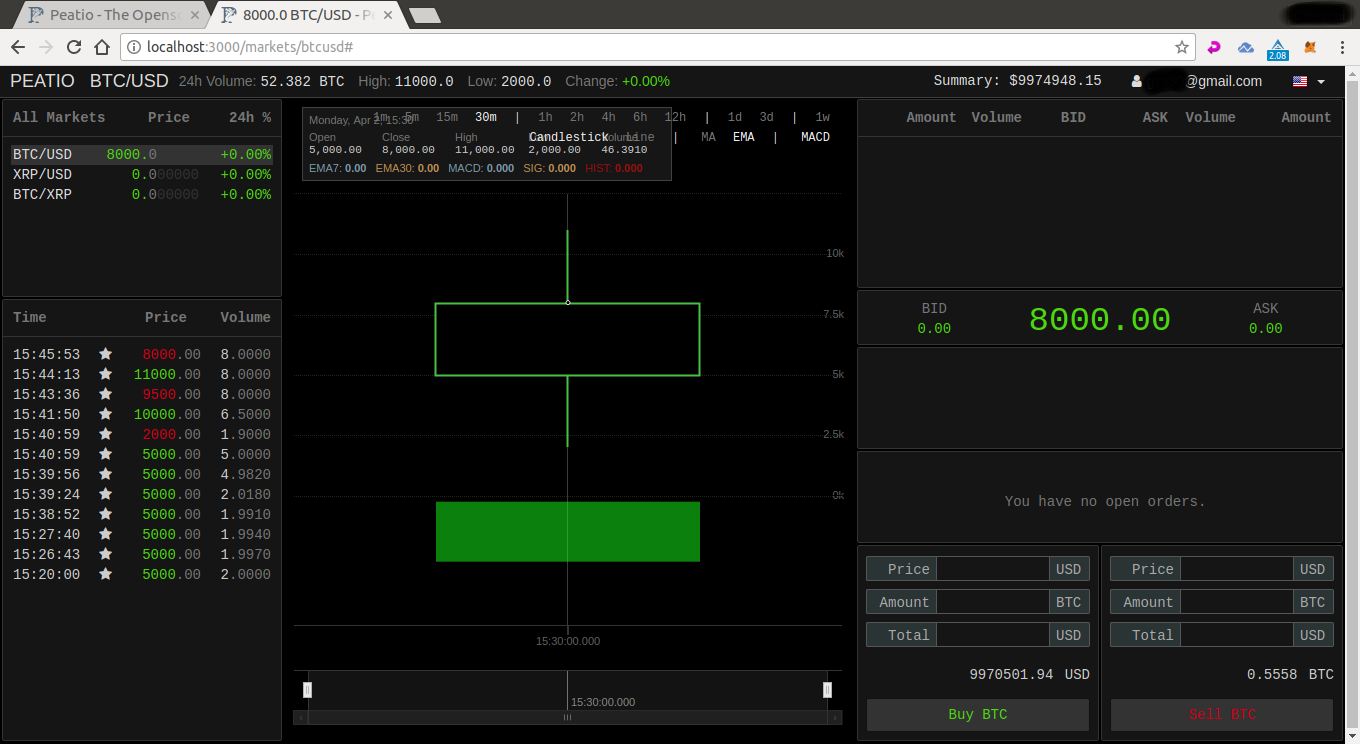
\includegraphics[width=\textwidth*2/3,height=\textheight,keepaspectratio]{RE_TradingUIC}
	\captionof{figure}{UI di trading di Ripa Exchange}
	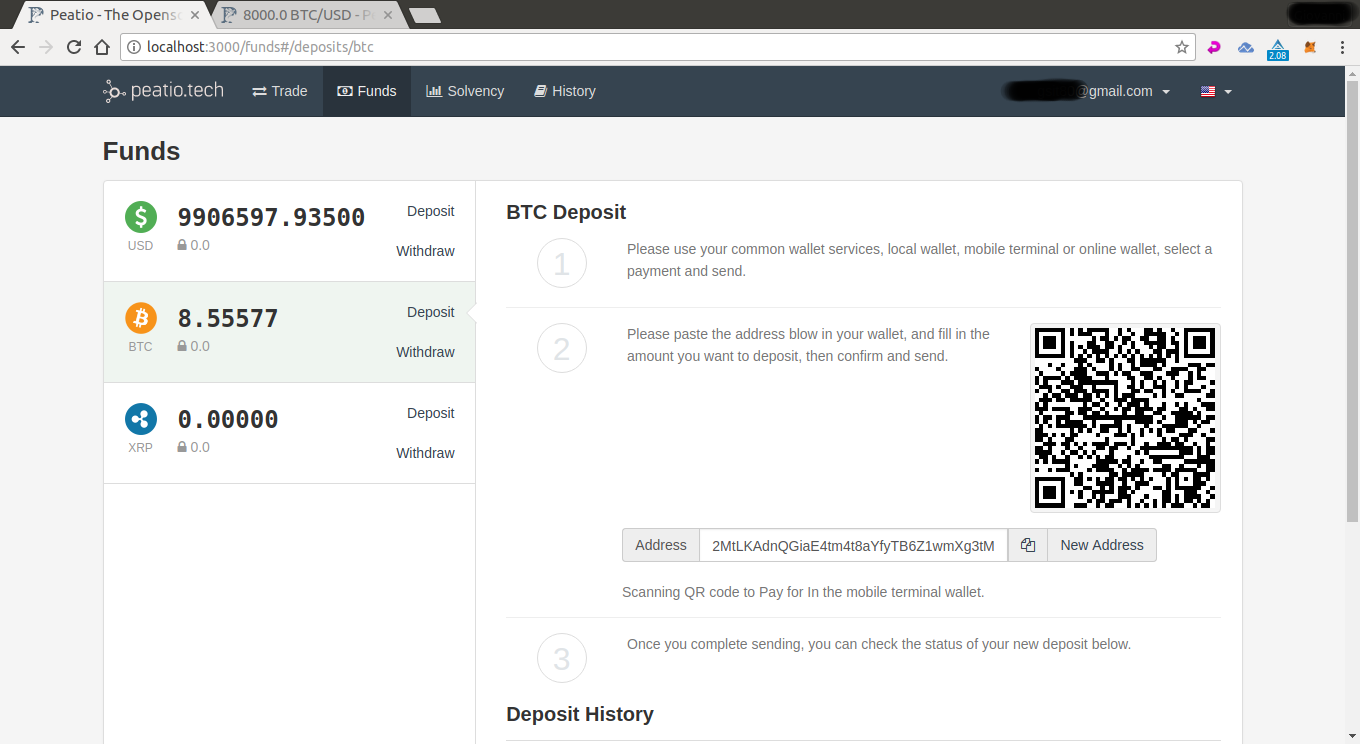
\includegraphics[width=\textwidth*2/3,height=\textheight,keepaspectratio]{RE_depositBTCC}
	\captionof{figure}{UI di deposio/prelievo}
	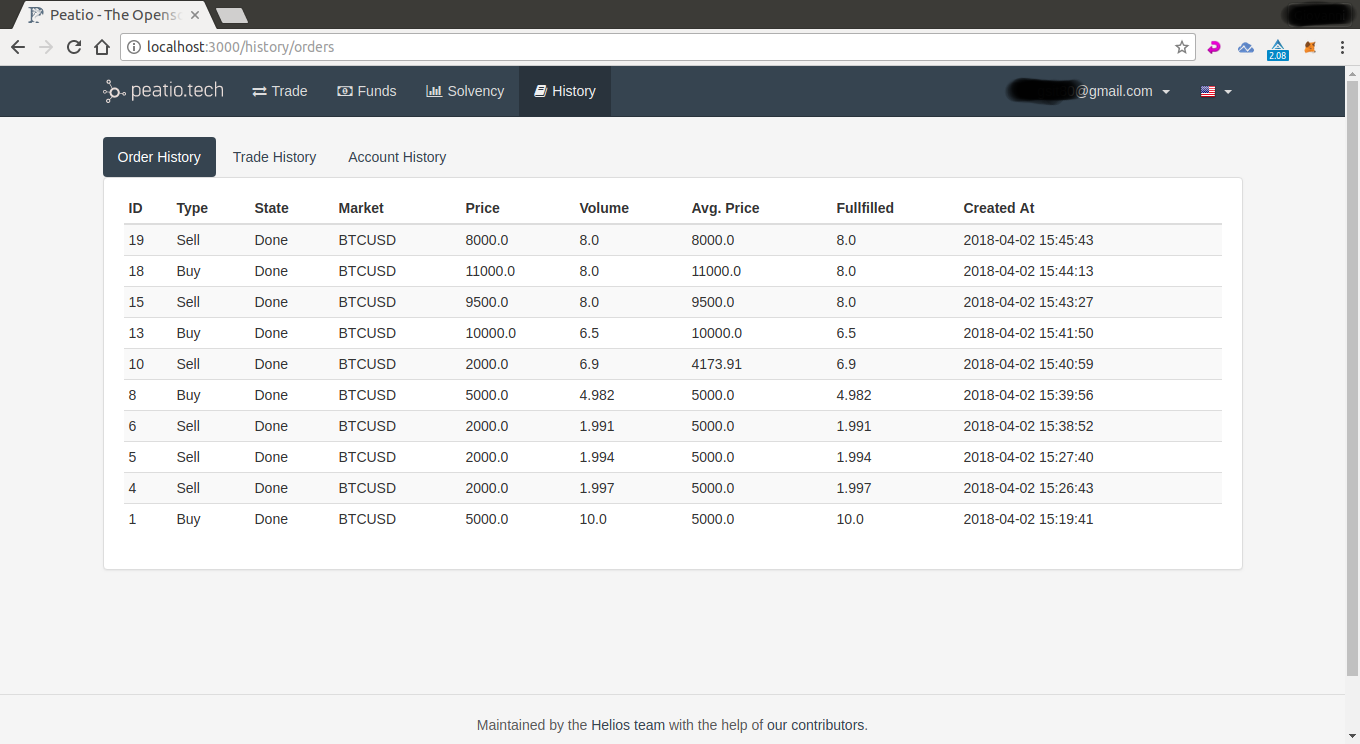
\includegraphics[width=\textwidth*2/3,height=\textheight,keepaspectratio]{RE_historyC}
	\captionof{figure}{UI di storico ordini}
	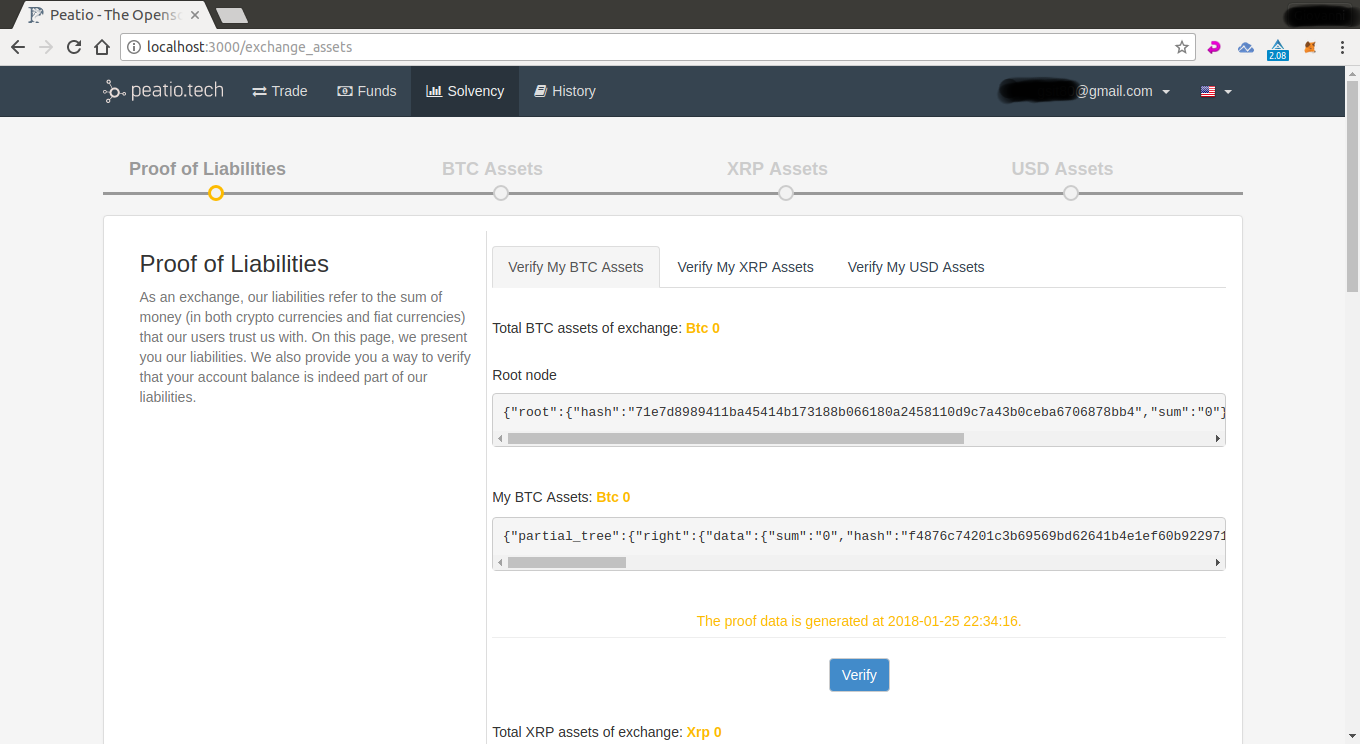
\includegraphics[width=\textwidth*2/3,height=\textheight,keepaspectratio]{RE_solvencyC}
	\captionof{figure}{UI di prova di solvibilità}
\end{center}

\subsection{Admin Interface}
Di seguito alcuni screenshot dell'interfaccia utente dell'area amministrativa dell'exchange Ripa:
\textcolor{darkred}{questi screenshot sono un lavoro in corso e non è detto che rappresentino l'interfaccia utente del prodotto finale}
\begin{center}
	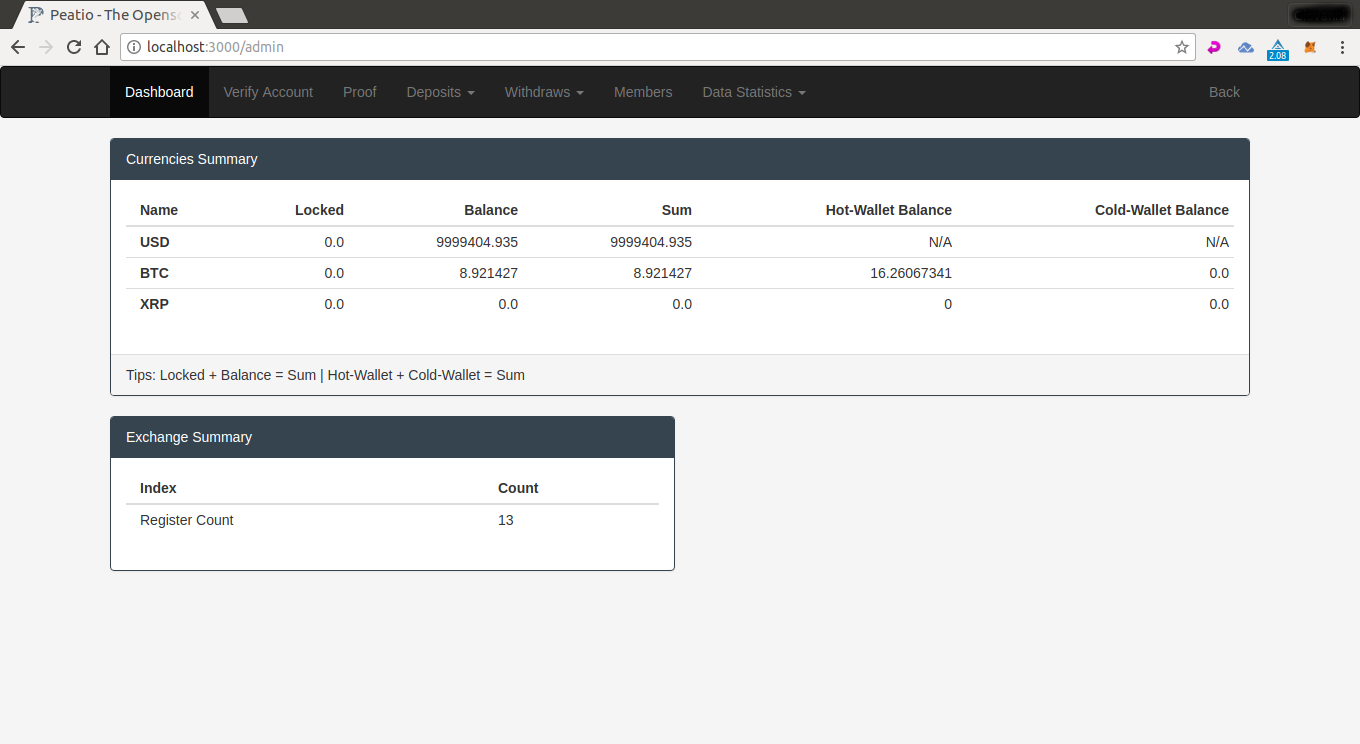
\includegraphics[width=\textwidth*2/3,height=\textheight,keepaspectratio]{RE_adminDashboardC}
	\captionof{figure}{Admin console dashboard}
	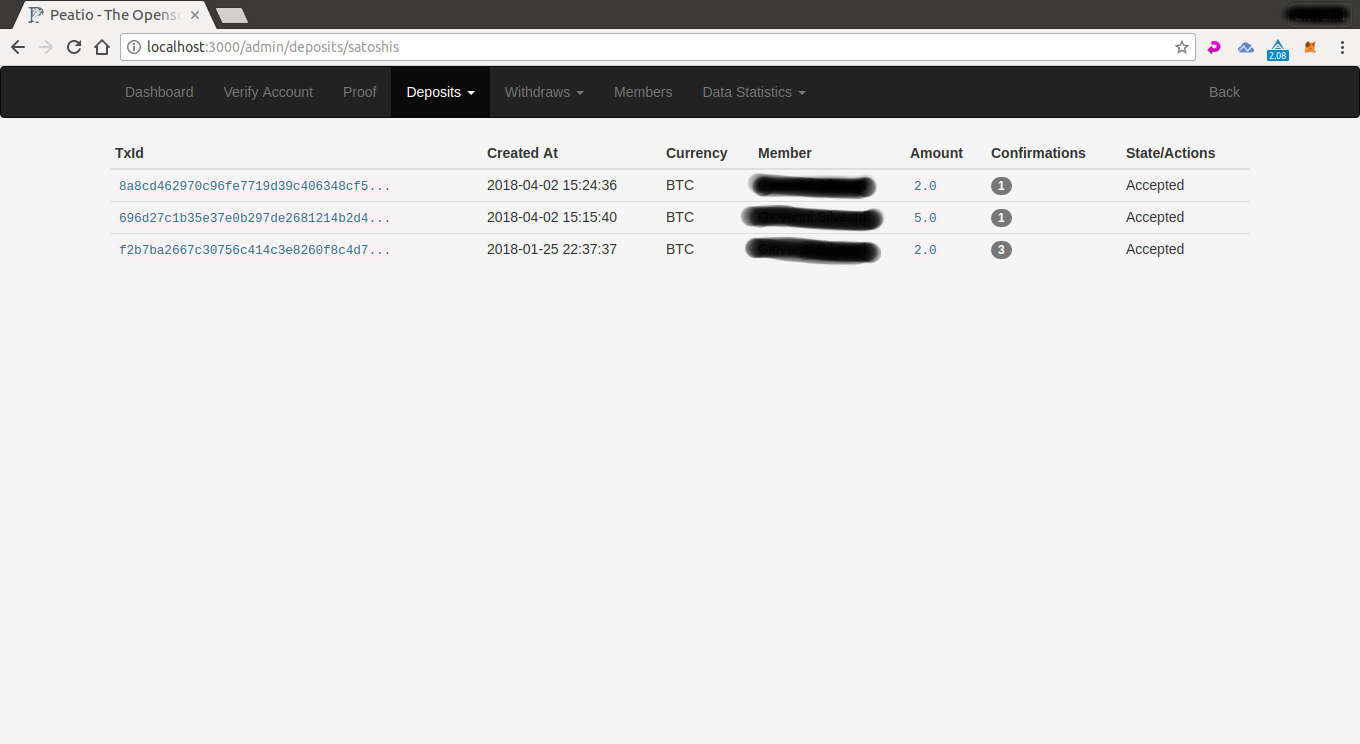
\includegraphics[width=\textwidth*2/3,height=\textheight,keepaspectratio]{RE_adminDepositsC}
	\captionof{figure}{Admin console sezione di deposito}
	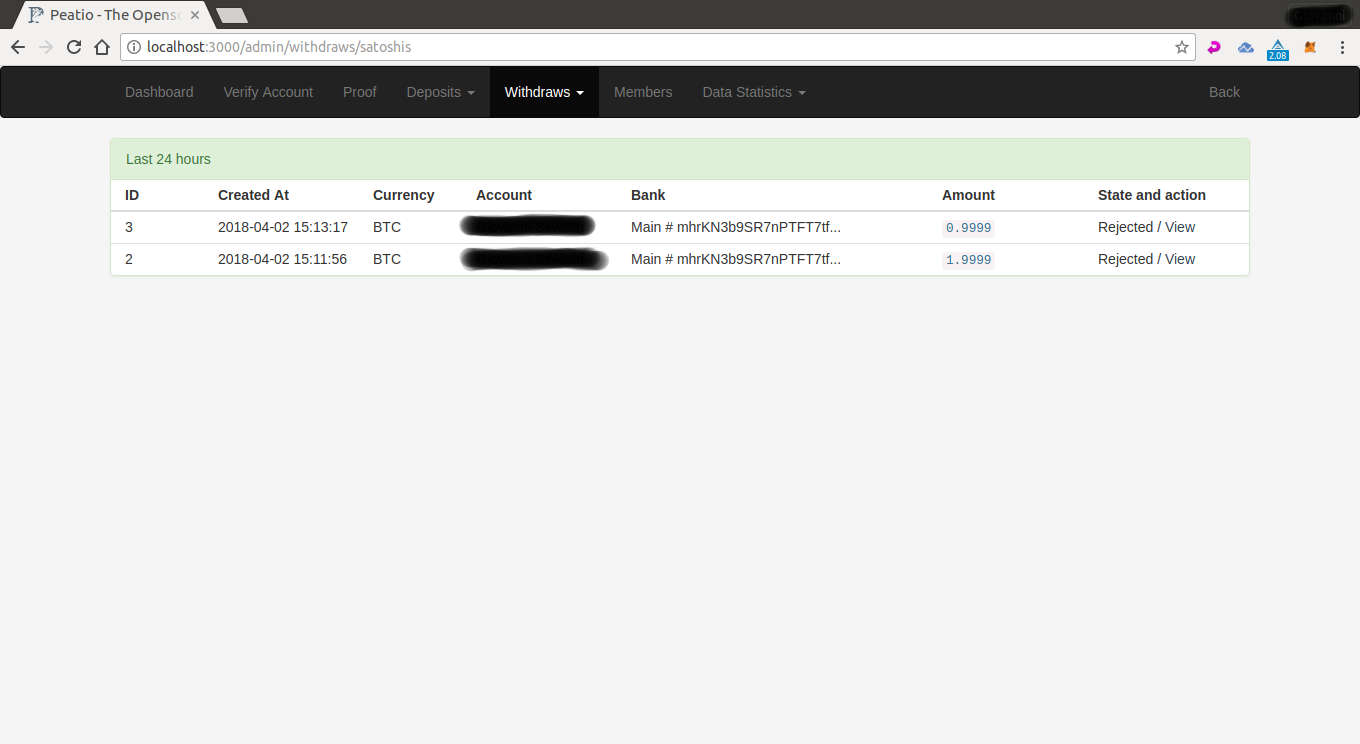
\includegraphics[width=\textwidth*2/3,height=\textheight,keepaspectratio]{RE_adminWithdrawsC}
	\captionof{figure}{Admin console sezione di prelievo}
	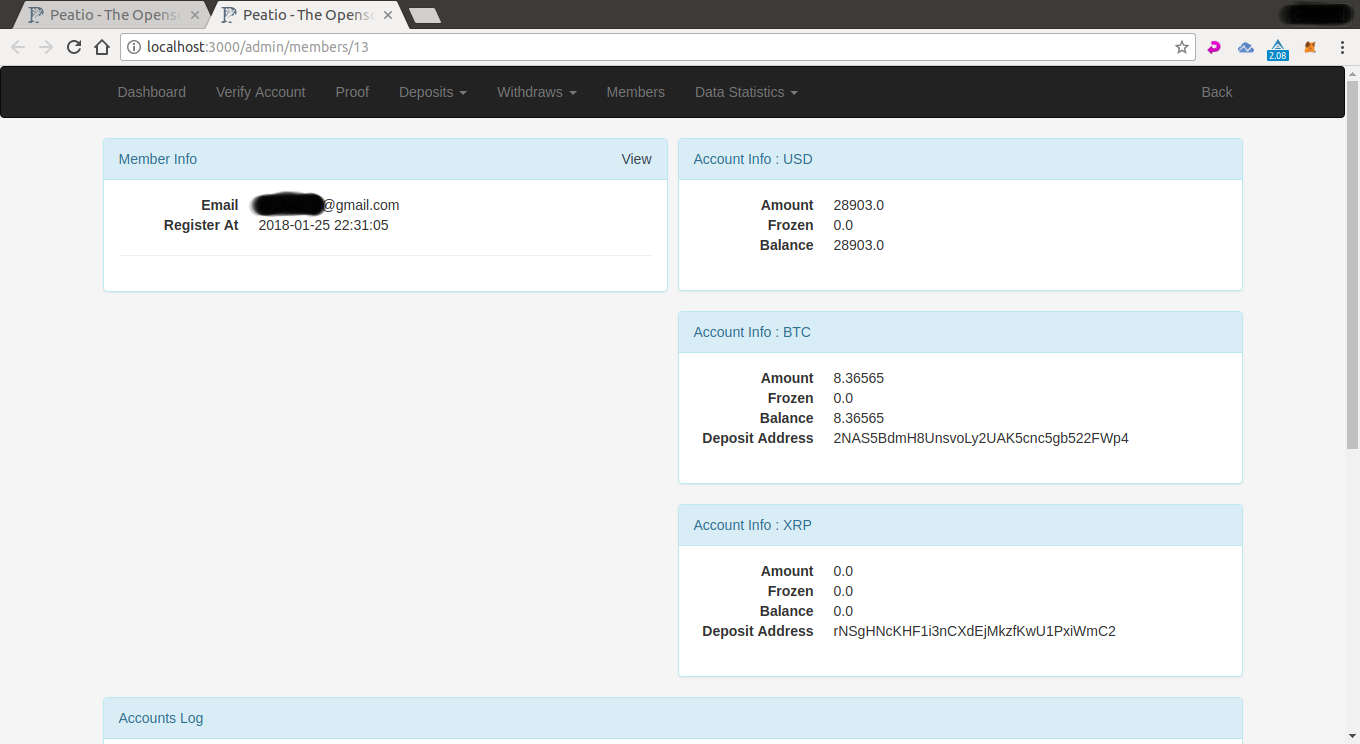
\includegraphics[width=\textwidth*2/3,height=\textheight,keepaspectratio]{RE_adminUserInfo1C}
	\captionof{figure}{Sezione informazioni utente}
	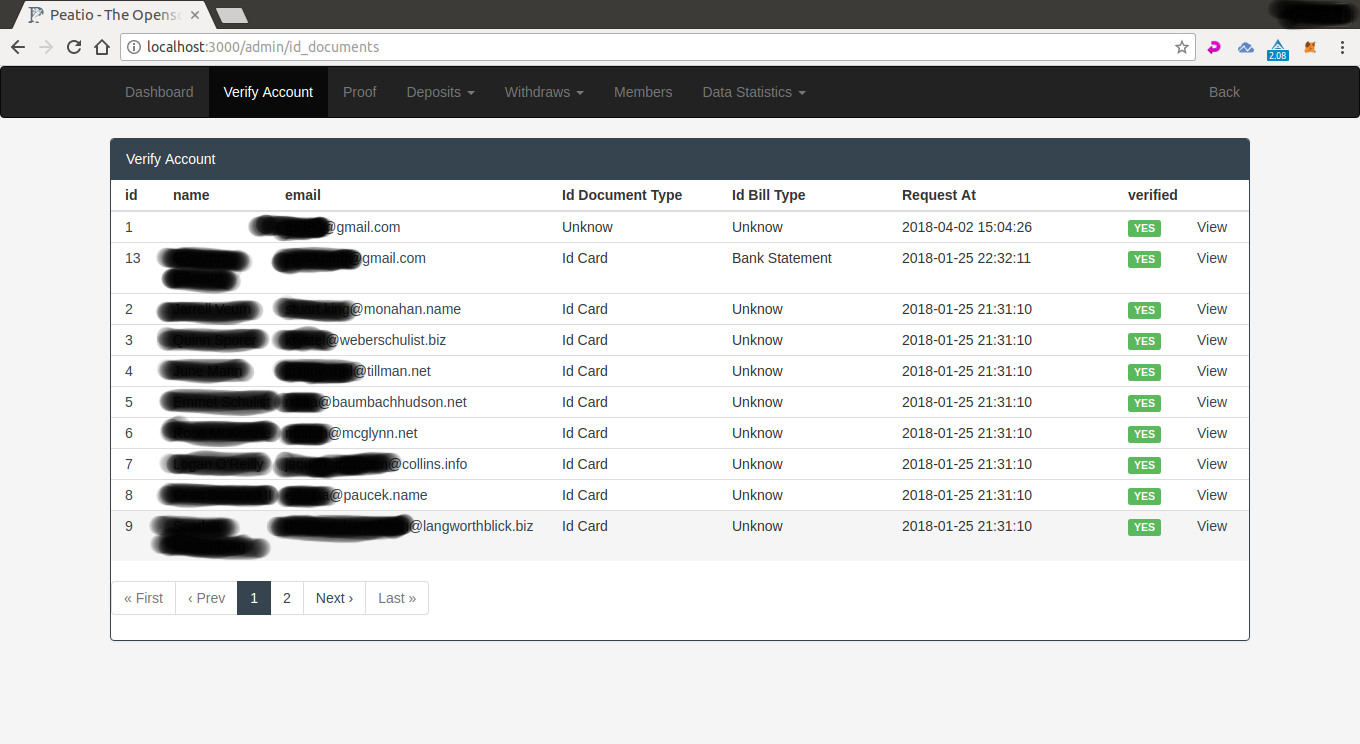
\includegraphics[width=\textwidth*2/3,height=\textheight,keepaspectratio]{RE_adminVerifyAccountC}
	\captionof{figure}{Sezione verifica utente}
\end{center}

\section{Funzionalità al Lancio}
All'apertura della prima istanza di Ripa Exchange le seguenti funzionalità sono previste:
\begin{itemize}
	\item \textsc{\textsc{CRYPTO $\Leftrightarrow$ CRYPTO}}: exchange di cambio valuta virtuale in valuta virtuale
	\item \textsc{\textsc{OAuth}}: Facebook, Google, Twitter
	\item \textsc{\textsc{FIDO}}: login con standard FIDO Alliance
	\item \textsc{\textsc{Protocolli}}: POW, DPOS, Masternode, tether, ERC20 accettati dall'exchange
	\item \textsc{\textsc{Valute}}: BTC, ETH, DOGE, BCH, TUSD, ARK, LISK, SHIFT, RISE, KAPU, OXY, RIPA, token ERC20 promettenti, 
	ed altre valute nella sezione protocolli non citate qui
	\item \textsc{\textsc{Mercati Principali}}: BTC, ETH, ARK
	\item \textsc{\textsc{Tipo di Ordini}}: market, limit
\end{itemize}

\subsection{Funzionalità Future}
Le future istanze di Ripa Exchange implementeranno le seguenti funzionalità:
\begin{itemize}
	\item \textsc{\textsc{E-Wallets}}: OKPay, NETELLER, MoneyPolo, others...
	\item \textsc{\textsc{Funzionalità di Trading Avanzate}}: margin trading, stop loss and take profit, 
	\item \textsc{\textsc{FIAT $\Leftrightarrow$ CRYPTO}}: depositi/prelievi tramite bonifico bancario
	\item \textsc{\textsc{Altre funzionalità}}: VISA/MasterCard, merchants tools, P2P Lending 
\end{itemize}

\section{Verso un Exchange Decentralizzato...}
Ripa Exchange è un exchange centralizzato che sarà convertito in un ibrido-decentralizzato per creare una rete di exchange
che condividono lo stesso codice sorgente e la stessa liquidità in modo tale che tu possa offrire liquitià ai tuoi clienti 
già dal giorno 1 di apertura degli scambi finanziari.\\

Per offrire i PRO di un exchange centralizzato come supporto di livello platino e scambio FIAT, ed i PRO di un exchange 
decentralizzato come la liquidità, senza i CONTRO di entrambi, dovremo eseguire questa passaggio con lo step intermedio di un exchange 
ibrido-decentralizzato e durante la fase 3 del progetto RipaEx (WP 4-6) esguiremo tutte le analisi funzionali e tecniche 
richieste per costruire il prossimo passo su fondamenta solide ed offrire alla comunità RipaEx un exchange open source, sicuro
ed efficiente.

